\section{Strategisk analyse}
\begin{figure}[H]
	\centering
	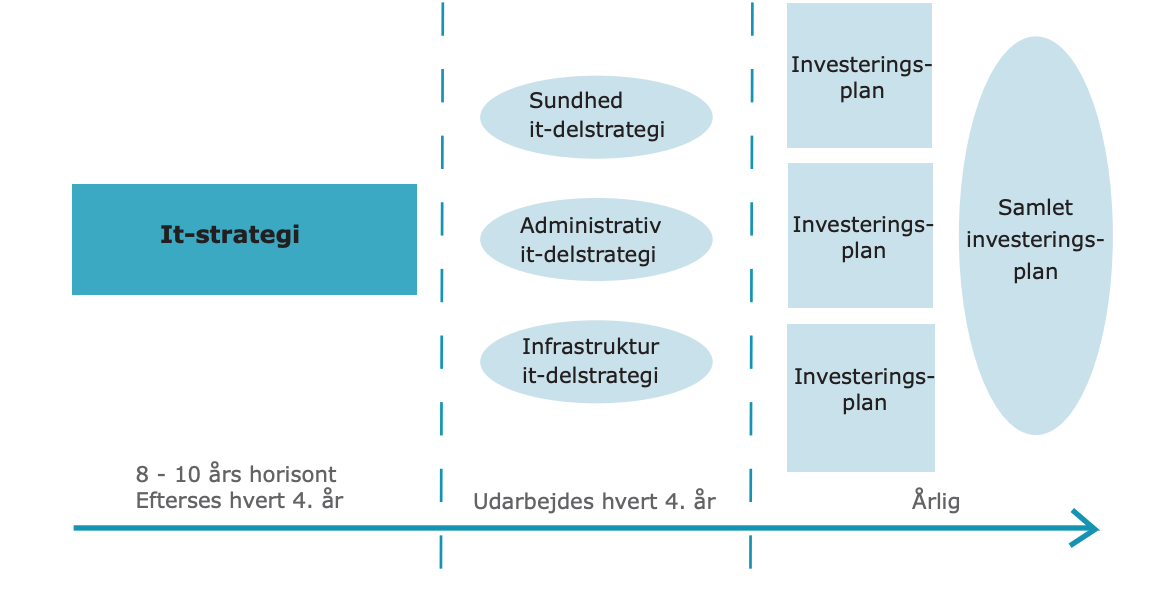
\includegraphics[width=\linewidth]{Materials/Strategy}
	\caption{It-strategien og de tilhørende it-delstrategier}
\end{figure}
Ovenfor ses Region Sjællands it strategi, og hvordan den er bygget op. Den overordnede it strategi udgør sammen med delstrategierne rammerne for investeringsplanerne som efterfølgende financierer strategierne. Som det ses er tidshorisonten for den overordnede it strategi på otte til ti år. Denne tilgang er taget for at sikre ambitionsniveauet for strategien kan realiseres over flere delstrategiperioder således at regionen løbende kan få et indtryk af den aktuelle situation.
\subsection{IT Strategien}
Nogle af de vigtigste målsætninger for den overordnede it strategi er:
\begin{enumerate}
	\item Regionen ønsker at skabe en sammenhængende og effektiv virksomhed gennem øget samarbejde både internt men også med samarbejdspartnere og borgere.
	\item Regionen vil have fuldt udbytte af sine investeringer, og de nye løsninger skal bruges i deres fulde omfang.
	\item Regionen vil begrænse risici involveret i at indføre nye it løsninger og vil derfor tage ved lære af andres viden og erfaringer. Det er derfor at foretrække hvis de nye systemer er efterprøvede af andre organisationer i eller uden for landet.
	\item De administrative og kliniske arbejdspladser skal have samlet adgang og samlet præsentation til al relevant data uanset kilde og teknologi. De skal have adgang fra en flerhed af mobile enheder. Der skal desuden være større anvendelse af data i eksisterende og kommende systemer.
	\item Regionen har en målsætning om at de administrative og kliniske arbejdspladser skal være papirløse. Dette skal realiseres ved at automatisere, forenkle og standardisere opgavevaretagelse.
	\item De løsninger som tages i brug skal være brugervenlige og intuitive.
	\item Regionen har en målsætning om at borgere, patienter,
	pårørende og samarbejdspartnere i så høj grad som muligt kan betjene dem selv uden at gå på kompromis med kvalitet og service. Målet er, at disse grupper skal opleve en bedre servicegrad, samtidig med at regionen reducerer sit ressourceforbrug.
	\item Regionen ønsker én arbejdsopgave til ét system. Men det er samtidigt vigtigt med systemer som kan hente information fra andre systemer.
\end{enumerate}
\subsection{Sundheds-it}
Nogle af de vigtigste målsætninger for sundheds it strategien er:
\begin{enumerate}
	\item Regionen har en målsætning om at give ensartede oplevelser og behandling uanset geografi.
	\item Regionen ønsker at den enkelte kliniker skal kunne få et samlet, mobilt og nemt tilgængeligt overblik over de opgaver og de patienter som den enkelte kliniker tildeles eller har kontakt til. I princippet skal en kliniker kunne
	trække 'glaspladen' op af lommen og få fuldt overblik over egne opgaver og alle relevante kliniske data og billeder fra alle systemer.
	\item Gennem implementering af it systemer ønsker regionen at understøtte driften og sikre effektivisering af ressourceanvendelsen.
	\item Telemedicin skal optimere patientforløb i forhold til accelerering, adgang til relevant ekspertise, diagnostik, behandling og kontinuitet. 
\end{enumerate}
\subsection{Administrativ-it}
Nogle af de vigtigste målsætninger for den administrative it strategi er:
\begin{enumerate}
	\item Regionen vil skabe en sammenhængende, effektiv og papirløs administration gennem automatisering, procesunderstøttelse og digitalisering af arbejdsgange.
	\item Regionen ønsker realtidsledelsesinformation som skal tage afsæt i driften.
	\item Regionens kommunikative mål er ensartethed uanset geografi og at de kommunikative it løsninger skal være mobile.
\end{enumerate}
\subsection{It-infrastruktur}
Nogle af de vigtigste målsætninger for it-infrastruktur strategien er:
\begin{enumerate}
	\item Regionens infrastruktur skal være sikker, enkel, let og stabilt tilgængelig og med ubegrænset kapacitet set fra brugerens synspunkt.
	\item Regionen vil løbende tage nye systemer i brug, og ønsker derfor løsninger som der kan udvides.
	\item Brugeren skal kunne finde løsninger i samme brugervendte arbejdsgange, uden at brugerne skal opleve behov for at navigere mellem forskellige løsninger. Regionen ønsker systemer som kan hente information fra andre systemer således at brugeren kun skal henvende sig et enkelt sted.
	\item Regionen ønsker integrerede selvbetjenings løsninger.
\end{enumerate}


Al information i kapitlet er taget fra Region Sjællands egen publikation af deres it strategi\footnote{\url{https://www.regionsjaelland.dk/publikationer/Documents/it-strategi-region-sjaelland.dk.pdf}}.

\subsection{Problemer og behov}
Ud fra de ovenstående mål, ser vi at regionen finder det problematisk at klinikere ikke har det store overblik ved hånden hele tiden. De ønsker løsninger som er mobile og kan skabe overblik på kryds af alle systemer. De møder problemer med ressourceallokering, og hvordan de effektivt benytter de ressourcer de har til rådighed.\\
De har behov for systemer som er sikre og intuitive for brugerne, og som brugeren selv kan betjene. De har behov for et samlet system hvor brugeren kan finde al nødvendig information. De har behov for systemer som er afprøvede og testede i drift. Der er behov for at de it løsninger som bliver taget i brug kan udvides.